%%%%%%%%%%%%%%%%%%%%%%%%%%%%%%%%%%%%%%%%%%%%%%%%%%%%%%%%%%%%%%%%%%%%%%%%%%%%%%%%
%2345678901234567890123456789012345678901234567890123456789012345678901234567890
%        1         2         3         4         5         6         7         8

%\documentclass[journal,transmag]{IEEEtran}% Comment this line out if you need a4paper

\documentclass[10pt, conference]{ieeeconf}      % Use this line for a4 paper

\IEEEoverridecommandlockouts                              % This command is only needed if 
                                                          % you want to use the \thanks command

%\overrideIEEEmargins                                      % Needed to meet printer requirements.

% See the \addtolength command later in the file to balance the column lengths
% on the last page of the document

% The following packages can be found on http:\\www.ctan.org
%\usepackage{graphics} % for pdf, bitmapped graphics files
%\usepackage{epsfig} % for postscript graphics files
%\usepackage{mathptmx} % assumes new font selection scheme installed
%\usepackage{times} % assumes new font selection scheme installed
%\usepackage{amsmath} % assumes amsmath package installed
%\usepackage{amssymb}  % assumes amsmath package installed

\newtheorem{theorem}{Theorem}[section]
\newtheorem{lemma}[theorem]{Lemma}
\newtheorem{proposition}[theorem]{Proposition}
\newtheorem{corollary}[theorem]{Corollary}
\usepackage[ruled,vlined]{algorithm2e}

\newcommand{\qed}{\nobreak \ifvmode \relax \else
      \ifdim\lastskip<1.5em \hskip-\lastskip
      \hskip1.5em plus0em minus0.5em \fi \nobreak
      \vrule height0.75em width0.5em depth0.25em\fi}

\def\lc{\left\lfloor}   
\def\rc{\right\rfloor}

\usepackage{amsmath,amssymb}

\usepackage{tabularx}
\usepackage{tikz,hyperref,graphicx,units}
\usepackage{subfigure}
\usepackage{benktools}

\usepackage{caption}
\usepackage{epstopdf}
\renewcommand{\captionfont}{\footnotesize}
\usepackage{sidecap,wrapfig}
\usepackage[ruled,vlined]{algorithm2e}
\DeclareMathOperator*{\argmin}{arg\,min}
\DeclareMathOperator*{\argmax}{arg\,max}
\newcommand{\abs}[1]{\lvert#1\rvert} 
\newcommand{\norm}[1]{\lVert#1\rVert}
%\newcommand{\suchthat}{\mid}
\newcommand{\suchthat}{\ \big|\ }
\newcommand{\ba}{\mathbf{a}}
\newcommand{\bb}{\mathbf{b}}
\newcommand{\bc}{\mathbf{c}}
\newcommand{\bd}{\mathbf{d}}
\newcommand{\bg}{\mathbf{g}}
\newcommand{\bj}{\mathbf{j}}
\newcommand{\bn}{\mathbf{n}}
\newcommand{\bp}{\mathbf{p}}
\newcommand{\bw}{\mathbf{w}}
\newcommand{\bt}{\mathbf{t}}
\newcommand{\bu}{\mathbf{u}}
\newcommand{\by}{\mathbf{y}}
\newcommand{\bx}{\mathbf{x}}
\newcommand{\bz}{\mathbf{z}}
\newcommand{\bbf}{\mathbf{f}}
\newcommand{\bzero}{\mathbf{0}}
\newcommand{\bG}{\mathbf{G}}
\newcommand{\bA}{\mathbf{A}}
\newcommand{\bW}{\mathbf{W}}
\newcommand{\bX}{\mathbf{X}}
\newcommand{\mX}{\mathcal{X}}
\newcommand{\mD}{\mathcal{D}}
\newcommand{\mG}{\mathcal{G}}
\newcommand{\mN}{\mathcal{N}}
\newcommand{\mW}{\mathcal{W}}
\newcommand{\mF}{\mathcal{F}}
\newcommand{\bZ}{\mathbf{Z}}
\newcommand{\mR}{\mathcal{R}}

\newcommand{\bfc}{W}
\newcommand{\Qinf}{Q_{\infty}}
\newcommand{\st}[1]{_\text{#1}}
\newcommand{\rres}{r\st{res}}
\newcommand{\pos}[1]{(#1)^+}
\newcommand{\depth}{\operatorname{depth}}
\newcommand{\dist}{\operatorname{dist}}
\newcommand{\convhull}{\operatorname{ConvexHull}}
\newcommand{\minksum}{\operatorname{MinkowskiSum}}

\newcommand{\specialcell}[2][c]{ \begin{tabular}[#1]{@{}c@{}}#2\end{tabular}}
\newcommand{\acro}{SHIV}
\newcommand\independent{\protect\mathpalette{\protect\independenT}{\perp}}
\def\independenT#1#2{\mathrel{\rlap{$#1#2$}\mkern2mu{#1#2}}}

\newcolumntype{L}[1]{>{\RaggedRight\hspace{0pt}}p{#1}}
\newcolumntype{R}[1]{>{\RaggedLeft\hspace{0pt}}p{#1}}


\newboolean{include-notes}
\setboolean{include-notes}{true}
\newcommand{\adnote}[1]{\ifthenelse{\boolean{include-notes}}%
 {\textcolor{green}{\textbf{AD: #1}}}{}}

\renewcommand{\baselinestretch}{.99}


%\title{Iterative Imitation Learning with Reduced Human Supervision [v11]}
%\title{SHIV:  Reducing Human Supervision for Robot Active Learning [v11]}

\title{SHIV: Reducing Supervisor Burden using Support Vectors to Efficiently Learn Robot Control Policies from Demonstrations}



\author{Michael Laskey$^1$, Sam Staszak, Wesley Yu-Shu Hsieh, Jeff Mahler, Florian T. Pokorny$^1$, Anca Dragan$^1$, Ken Goldberg$^2$% <-this % stops a space
\thanks{$^1$Department of Electrical Engineering and Computer Sciences; {\small \{mdlaskey, ftpokorny, anca\}@berkeley.edu}}%
\thanks{$^2$Department of Industrial Engineering and Operations Research and Department of Electrical Engineering and Computer Sciences; {\small goldberg@berkeley.edu}}%
\thanks{$^{1-2}$ University of California, Berkeley;  Berkeley, CA 94720, USA}%
} 

\begin{document}



\maketitle
\thispagestyle{empty}
\pagestyle{empty}


%%%%%%%%%%%%%%%%%%%%%%%%%%%%%%%%%%%%%%%%%%%%%%%%%%%%%%%%%%%%%%%%%%%%%%%%%%%%%%%%

\begin{abstract}
The SHIV algorithm proposes an alternative to previous query selection methods for stream-based active learning to the non-stationary distributions encountered in robot control.  To reduce operator burden, the Svm-based reduction in Human InterVention (SHIV) algorithm only requests supervision for sufficiently risky or novel states.

In traditional imitation learning, a human expert provides a few demonstrations to the robot, which then \emph{offline} learns a policy to extrapolate these examples to new situations. One challenge is that during execution of the learned policy, a small but inevitable error will amplify, taking the robot further and further away from the regions of state space for which it has seen examples. 

\emph{Online} imitation learning algorithms such as DAgger address this challenge by iteratively executing a trained policy, and asking the expert for additional examples along the states visited by that policy. Such algorithms perform well in new situations, but rely much more heavily on extensive human supervision.

Our goal is to reduce the amount of human supervision required in imitation learning, without sacrificing performance. \emph{Our key insight is that the robot should ask for supervision only when its current trained policy has high risk.}

We introduce a method for online imitation learning that evaluates risk based on novelty of a state, as well as prior difficulty in labeling a nearby states. Our algorithm, SHIV (SVM-Based Reduction in Human Intervention), follows the trained policy when evaluated risk is low, and asks for human supervision otherwise. Our experiments with a toy car domain, as well as with non-prehensile grasping in clutter, suggest that our method can better utilize a human supervision budget, achieving higher success rates for the same number of queries to the expert.



%A trained policy can have a high risk of predicting the wrong action for a state for two reasons: 1) the state is too far away from the training states, and 2) the state is in an area in which the learner has historically struggled. We introduce a method for iterative imitation learning that estimates regions of high risk based on these two criteria, and limits queries to the supervisor to only high risk states. Our method instantiates stream based active learning, with a query selection strategy that generalizes novelty detection to querying in areas that are inherently difficult to correctly label.

% \adnote{Old abstract:}


% For robot control problems where the reward function  and the dynamics of the environment are not specified, the
% learning from demonstrations approach provides an algorithmic paradigm for learning a policy from supervisor-provided
% demonstrations. Dataset Aggregation (DAgger) in particular yields a state of the art method in this context which treats
% the problem of determining a policy as an iterative supervised learning problem which alternates between executing a
% trained policy and acquiring new supervisor control inputs for roll-outs of a current best policy estimator. In this
% work, we propose a novel algorithm, \acro~which is based on DAgger and which estimates the riskiness of states
% encountered by the policy roll-outs by means of an approximate quantile super-levelset estimate of the distribution of
% states used for training the current policy. Since learning a quantile function for high-dimensional input data is
% challenging, we instead modify an SVM-based approach to quantile estimation that employs regularization to solve this
% problem approximately. Our algorithm considers roll-outs with early termination as soon as a state outside a
% user-defined quantile super-levelset is encountered. Our approach furthermore reduces the amount of neccessary
% supervisor demonstrations by only collecting supervisor control inputs at states outside the current quantile estimate.
% In experiments involving a simulated race track and in a Super Mario Atari game benchmark considered by the authors of
% DAgger, our approach results in similar performance levels as DAgger while reducing the amount of required supervisor
% control inputs by more than {\color{blue}[-- TODO --]} percent.
 \end{abstract}


%%%%%%%%%%%%%%%%%%%%%%%%%%%%%%%%%%%%%%%%%%%%%%%%%%%%%%%%%%%%%%%%%%%%%%%%%%%%%%%%

\section{Introduction} 


We focus on \emph{model-free imitation learning} problems. In this problem domain, the robot learns a task, such as grasping an object while pushing clutter out of the way \adnote{we need to put this in fig 1 and refer to it here}, from \emph{examples} provided by a human \emph{expert}. The robot does not have direct access to a reward function that describes the task, nor to a dynamics model informing it how its actions will affect the world.

Thus, to achieve the task, the robot directly learns a \emph{policy}, mapping states (or in some cases observations) to actions, which eliminates the need for a reward or a model. It does this based on examples, which are state-action pairs performed by the expert while demonstrating the task (see section 4.1 of \cite{argall2009survey}  for more details).

Traditional approaches work \emph{offline}, passively receiving examples from the expert first, and then approximating a state-action mapping in a second phase. One challenge that these approaches face is that when the robot is executing its trained policy, its actions affect the resulting next state. That makes the visited states not independent random variables. The practical consequence is that small but often inevitable differences from the supervisor's policy cause the sequence of visited states to drift far from the region of space where the robot has seen training examples, leading to poor performance. 

For example, when training an autonomous car to drive on the highway, the car will deviate form the middle of the road and will not be able to recover, because all the training examples are from the middle of the road \cite{pomerleau1989alvinn}. Theoretically, the number of mistakes made by the robot in such cases may not scale just linearly, but \emph{quadratically} with the time horizon of the task \cite{ross2010efficient}.

\begin{figure}[t!]
\centering
\includegraphics[width=\columnwidth]{figures/teaser.pdf}
\caption{ 
Given a set of states corresponding to images of a race-track simulation (visualized in $\mathbb{R}^2$) with expert
control inputs, we consider a quantile super levelset estimate (shaded) as an approximation of the riskiness of
executing the trained policy at a given state. By varying the quantile threshold, we can increase or decrease the size
of the quantile super-levelset area. In our approach, points outside the super-levelset are considered risky and, during
training, roll-outs of the policy that leave the super-levelset require control demonstrations from the supervisor,
while roll-outs within the super-levelset can be performed autonomously. 
}
\vspace*{-10pt}
\label{fig:dis_traveled}
\end{figure}

\emph{Online} imitation learning approaches address this by iteratively gathering more examples form the expert \cite{grollman2007dogged,ross2010efficient,ross2010reduction}. DAgger is such an algorithm, and works by training a policy on existing examples, but then ``rolling it out'' (execute it) to see what states are likely to occur under this new policy. The expert then provides examples in the new states, correcting the robot's policy, and these examples are aggregated with the previous ones in a training set for the next iteration. 

With such algorithms, the number of mistakes has indeed been proven to scale only linearly with the time horizon, as opposed to quadratically \cite{ross2010efficient}. DAgger and related algorithms have seen a wide range of applications, from quadrotor flight to natural language to Atari games~\cite{NIPS2014_5421,duvallet2013imitation,ross2013learning}.

On the other hand, online algorithms also place significantly more burden on the expert. DAgger requires the expert to manually provide controls or actions that the robot should have taken for each and every state it visits when rolling out the current best policy estimate. 

Our goal is to reduce the burden on the expert without harming performance, by more carefully selecting when to ask for examples:
\begin{quote}
\emph{The robot should not bother the human expert when its policy has low risk of error. Instead, it should only ask for new examples in regions of high risk.}
\end{quote}

States can have high risk for two complementary reasons: (1) they are far from the training examples --- this type of risk is studied under novelty or outlier detection \cite{hodge2004survey}; or (2) they lie in a region that has proven to be difficult to correctly label in the past, despite there being training data in that region.

Our main contribution is integrating this notion of risk into online imitation learning. We introduce SHIV (), which builds on the One Class SVM method for approximating quantile level sets \cite{scholkopf2001estimating} to evaluate this risk. 

We analyze our algorithm on a car track example, studying the risk evaluation method along with its robustness to the selection of a threshold for how risk adverse the robot should be. We also compare it with state of the art online imitation learning on a more complex task of nonprehensile grasping in clutter. Our results suggest that SHIV learns policies with higher success rates for the same budget of expert examples. 

Overall, our work enables robots to actively decide when to ask for examples during online imitation learning, reducing the burden on the user and paving the way towards more effective human-robot interactions.





% \adnote{Old intro:}

% Consider the problem of teaching a robot a complex task such cooking a meal or as racing a toy car around a track
% against human opponents. When the robot is only provided with visual demonstrations without the knowledge or an
% underlying cost function describing the task, traditional model based control approaches are often not applicable. In
% these situations, the learning from demonstrations (LfD) approach provides a paradigmn for teaching a robot how to
% accomplish the task \cite{ross2013learning,pomerleau1989alvinn,schulman2013case}.\adnote{these are very random things to cite for LfD, FYI - there is a survey by Argall that usually gets cited}

% One approach to LfD is to train a policy, or a function estimator (either a classifier or regressor), to predict a
% supervisor's behavior given training data consisting of pairs of observations (input) and actions (output) performed
% while accomplishing a task. Since the robot's actions typically affect the resulting next state, the resulting sequences
% of states encountered during the execution of a policy are not independent random variables, thus making statistical
% inference challenging. Ross et al. proved that this can cause the error in the policy estimator to compound over the
% time and lead to performance degradation that is proportional to the time horizon of the task squared. The intuition
% behind this result is that as the robot makes mistakes with respect to the supervisor's policy it drifts from the
% distribution it was trained on and might encounter new states it can't generalize to.  Ross and Bagnell overcome this by
% presenting an iterative method that first trains a policy on the data observed using standard supervised learning
% techniques then tries (or 'rolls out') the policy out in the environment to see what states are likely to occur under
% the robot's trained policy.  The supervisor then tells the robot what controls it should applied after each iteration
% and the policy is retrained \cite{ross2010reduction}. The DAgger method has been successfully used since to teach a
% robot how to follow verbal instructions, achieve state of the art performance on Atari games and fly a quad copter
% through a forest~\cite{NIPS2014_5421,duvallet2013imitation,ross2013learning}.






% During learning, implementations of DAgger require the supervisor to manually provide control inputs that the robot
% should have applied for each states it visits when rolling out the current best policy estimate. If the supervisor is a
% human or an algorithm with a high time complexity, this can be tedious and expensive. We are hence interested in
% reducing the burdon on the supervisor by partitioning the state space into states where the policy can either be
% executed autonomously with little expected risk, or where supervisor control input (or 'labels') are likely to be
% required due to high 'risk'. A state can be risky for 2 reasons: 1) we encounter a state which has a low density of
% training data in its vicinity, which potentially means our policy will mis-predict the supervisor
% \cite{tokdar2010importance} 2) the state is near previously visited states, but the control-input is mis-predicted
% nonetheless. If an accurate density estimation corresponding to
% the pairs of visited states and control signals is available, the first scenario can be captured by regions of
% state-space with a low density estimate. Areas of low density are then considered to be risky since an insufficient data
% is available to accurately model the demonstrator's policy. This idea is also captured in the notion that 'a trained
% model will be able to generalize within the distribution it is trained on' \cite{tokdar2010importance} in statistical
% machine learning. The second case arises for example when the current best policy estimate is locally inconsistent with expert
% demonstrations.
% %
% %Vague!!!
% %This property can be seen used in importance sampling when data is collected from one distribution, but tested on
% %another and has to be re-weighted %to the test distribution \cite{huang2006correcting}. 
% %
% While the amount of data needed to accurately estimate the density increases exponentially with the dimension of state
% space \cite{nadaraya1964estimating}, we can turn to approximate methods which instead attempt to learn an approximate
% representation of the quantile levelsets of the distribution. Thus, we propose using a modified version the One Class
% SVM method for support estimation that only tries to estimate the level set of the quantile function of the density
% \cite{scholkopf2001estimating} at a user-determined quantile threshold which has been used even with high-dimensional
% image data \cite{liu2014unsupervised}. Our modification furthermore removes areas of state space from the super-levelset
% estimate where the local policy estimate is inconsistent with the expert demonstrations.

% To apply our approach, we make the same assumptions as in the case of DAgger: 1) we require access to an environment
% where a robot can try out (roll out) policies to sample trajectories and where we are able to collect observation states
% and corresponding control inputs along these trajectories. 2) an interface allowing a supervisor to provide control
% inputs that should have been applied for states along parts of the rolled out trajectories. 3) We assume that we are
% able to collect a series of observations from the environment and the controls applied. 4) Lastly, for our theoretical
% analysis to apply, we assume the current observation only depends on the previous observation and control input (i.e.
% the Markovian assumption).

% Our core contribution is the extension of DAgger to \acro~which incorporates a notion of risk to learning from
% demonstrations and reduces supervisor
% burdon by asking for supervisor demonstrations only in `risky' states. 
% We achieve this by proposing a modified version of the One Class SVM, that both estimates the quantile level sets 
% of the distribution of states with demonstrations and additionally
% and carves out areas in the support where we know our policy will mis-predict the supervisor, thus identifying states of high
% risk.  Our experimental results on a Super Mario Atari video game,  suggest \acro~is able to reach DAgger's
% peak performance of surviving for an average of 2200 simulation steps with only 1200 queries to the supervisor, while DAgger required 2800 queries
% averaged over 20 levels.
% {\color{blue}[-- FINALIZE --]}

\section{Related Work}

Work related to ours can be grouped in two categories: work related to the active learning aspect, and work related to the risk evaluation aspect. 

\noindent\textbf{Active Imitation Learning.}
SHIV instantiates \emph{stream-based} active learning ~\cite{atlas1990training,cohn1994improving}, it receives the stream of states induced by executing the current best policy estimate, and actively decides for each state whether to query the expert or not.

Stream-based active learning has two ingredients: a stream, given here by the policy, and a query selection method. Typical query selection methods are estimator-centric: they evaluate the estimator's confidence (e.g. distance from the classification hyperplane \cite{tong2002support}), implicitly assuming a fixed distribution --- that the new data is sampled from the same distribution as the previous training data. Although such methods have been proposed for online imitation learning (see dogged learning \cite{chernova2009interactive,grollman2007dogged}),
online imitation learning violates the fixed distribution assumption because each new policy induces a new distribution of states . Another way to measure confidence is query by committee, which uses a committee of hypothesis classifiers that are trained on different subset of training data and only labels points for which they disagree. Judah et al. has proposed using this approach towards online imitation learning\cite{judah2011active,judah2012active}, however it has been shown when training and test distributions are different this can perform worse than randomly selecting points \cite{burbidge2007active}.


Instead, we contribute a query selection method that is data-centric, evaluating confidence based on novelty
and on historically mislabeled regions. %Our approach builds on the One Class SVM method for approximating quantile level sets \cite{}, which has already been used in novelty detection on high-dimensional image data \cite{}. 
Our results suggest that this method is a better predictor of misclassification risk than a typical, estimator-centric query selector.


\noindent\textbf{Risk via Novelty Detection.}
One part of our risk definition is the notion that a trained model will be able to generalize within the distribution it is
trained on \cite{tokdar2010importance}. Novelty detection \cite{hodge2004survey} is concerned with recognizing that a sample is outside of this distribution, making it difficult for a model to correctly predict its label.
One approach to novelty detection is to directly estimate the underlying probability density function from which the data is sampled. However, the amount of data needed to accurately do so scales exponentially in the number of dimensions \cite{nadaraya1964estimating}.

An alternative to evaluating the probability of a data point is to measure distance to its nearest neighbors \cite{knox1998algorithms}. However, this approach was shown to be
susceptible to outliers since nearest neighbors mostly incorporate local information about the data \cite{hodge2004survey}.

Our approach is based on the One Class SVM proposed by Scholk{\"o}pf et al., which estimates a particular quantile level set for the training data by solving a convex quadratic program  to find support
vectors. The method has been theoretically shown to approximate the quantile levelset of a density estimate
asymptotically for correctly chosen bandwidth settings and in the case of a normalized Gaussian kernel function \cite{vert2006consistency}. 
In \cite{liu2014unsupervised}, the One Class SVM has furthermore been used for novelty detection in high-dimensional 
image data.

% The field of learning from demonstrations has achieved state of the art performance in a variety of areas within robotics
% \cite{argall2009survey}. Abbeel et al.~used an iLQR controller based on helicopter trajectories demonstrated by a human expert
% to successfully learn a series of aerobatics stunts \cite{abbeel2007application}. Billard and Matari used a hierarchy of
% neural networks on video data and tracking markers to imitate the movement of human arms on a 37 degree of freedom humaniod
% robot \cite{billard2001learning}. Schulman et al. used a non-linear warping technique based on thin-plate splines
% to transer demonstrations of a human controlling a PR2 robot to tie knots with a rope to new and unseen initial
% configurations of the~\cite{schulman2013case}. 

% A subset of research in the field of learning from demonstrations is working within the assumptions that the dynamics of
% the robot and the environment are not known and that no access to a cost function describing a given task is available.
% Under these assumptions, a set of trajectories and controls can be collected from a supervisor and the policy learning
% problem can be treated as a supervised learning problem that determines a function from state space to
% controls~\cite{argall2009survey} by means of regression. Pomerleau et al. used this approach on raw image data and
% associated control inputs provided by a person driving a car. The authors then learned a policy that allowed a car to
% travel on a highway. However, they observed that if the car deviated from the middle of the road the learned policy was
% not able to recover, this behavior was attributed to the fact the car only drove in middle of the road while collecting
% demonstrations~\cite{pomerleau1989alvinn}. Ross et al. studied this effect and showed that error can accumulate at a
% rate quadratic in the time horizon of the policy in general. Ross et al. then proposed a learning algorithm, SMILE, that
% stochastically mixes the supervisor's control with the robot's policy control signal during training, thus allowing the
% robot to explore states the supervisor had not visited during training~\cite{ross2010efficient}. 

% Ross and Bagnell improved upon this method with DAgger (Dataset Aggregation) -- an iterative method that first trains a
% policy on the data observed using standard supervised learning techniques and then tries, or 'rolls out' the policy in
% the environment to see what states are likely to occur under the policy. The supervisor then tells the robot what
% controls it should applied at each stage of this roll-out and the policy is retrained with an aggregate of all data seen
% before \cite{ross2010reduction}. This algorithm has found widespread adoption in the robotics community. in
% \cite{ross2013learning}, a quad-copter using DAgger learned how to fly through a forest using only Histogram of Gradient
% (HOG) features extracted from camera images \cite{ross2013learning}. Guo et al. combined DAgger with Deep Q-learning
% methods to achieve state of the art performance on a common Atari game benchmark in Reinforcement Learning
% \cite{NIPS2014_5421}. Duvallet et al. furthermore used DAgger to teach robots to follow verbal instructions about where
% to move sematically in a building with a training set consisting of of humans following similar verbal instructions
% \cite{duvallet2013imitation}. Levine et al. very recently extended the iterative learning paradigm through Guided Policy
% Search, which replaces the expert with iLQG and uses KL-divergence constraints to train the policy~\cite{levine2015end}.  


% One limitation of DAgger which we address in the present work is that it requires the demonstrator, or supervisor, to
% provide control inputs that the expert would have applied for every state encountered along a roll-out of a trajectory at every interation of the
% algorithm. Providing these control inputs can be very tedious or expensive both in the case where the `supervisor' is a
% human or an algorithm with a high computational demand.

% In prior work, Judah et al. proposed applying active learning techniques to improve the learninng ability of an algorithm given a fixed budget. 
% \cite{judah2011active,judah2012active}. A drawback of this approach is that it requires us to estimate a complete
% density of states from the samples, which can be difficult especially in high dimensions. Furthermore, the  
% at each iteration only one labeled state was given. Thus, the robot could potentially be required to try out many more iterations of learning in order to successfully accomplished the task.  

% \begin{enumerate}
% \item Our work is different than traditional pool base active learning for two reasons 1) the data comes in as a stream (i.e. we decided whether to label or not label the sample vs. using a pool base methods) 2) the estimator being trained is part of the parametrization of the distribution of states being encountered at run time, thus violating the i.i.d assumption common in these methods. 
% \item Some techniques that can handle these approaches are 1) uncertainty sampling , or measuring some confidence level in a classifier and deciding whether to label or not. 2) Query by committee, which involves sampling a committee of hypothesises from a version space of consistent classifiers 3) Density weighted model, which fitting a density to the unlabeled pool and then using a technique such as uncertainty sampling or query by committee to chose the label with the highest uncertainity times the density under the model. The reason for density weighted model is because the previous approaches are prone to labeling outliers \cite{settles2008analysis}. 
% \item Our approach can be considered a query selective strategy that uses the ideas of density weighted models. The level set estimation of the One Class SVM is a binary decision metric of how close a point is to the global support points that define its neighbors. Then our hole punching technique places a "prior" on points that are likely to be misclassified condition on the fact that points nearby are misclassified. Thus, encapsulating both a notion of uncertainity and distance to relative points. 
% \item One point that I've been thinking about is that traditional active learning is about training an estimator on some fix distribution and then trying to predict how the estimator will change given new points sampled from the same distribution. Thus most approaches work on the estimator themselves (query by committee sampling different hypotheses or uncertainty sampling measuring confidence). This assumption is violated in DAgger because you are sampling from a new distribution each iteration different from what is trained on. Thus, a confidence threshold such as (distance to hyperplane for an svm) would be misleading because if the point was drawn from a different distribution it could be very far from the hyperplane, but have a different label than that side of the hyperplane. Thus, we purpose not looking at the estimator but at the data itself. We make an assumption that points close to other points in our feature space will have similar labels, but the outliers are unknown and will need new labels. I suggest we run a uncertainty sampling technique vs. SHIV to verify all this. 

% \end{enumerate}



% %[Let's discuss this part]
% {\color{blue}[-- IMPROVE THIS PARAGRAPH --]} In order to determine state space regions where a policy is likely to determine
% an incorrect control input, we leverage a
% property in statistical machine learning that a trained model will be able to generalize within the distribution it is
% trained on \cite{tokdar2010importance}. This property is used in importance sampling when data is collected from one
% distribution, but tested on another and has to be re-weighted to the test distribution \cite{huang2006correcting}. One
% approach is to estimate the probability density of states the policy is trained on. However, the amount of data needed to accurately estimate the density scales exponentially in the number of \cite{nadaraya1964estimating}.

% Several alternative approaches have been proposed to determine regions of state-space where an estimator is likely fail
% to generalize away from the training-data \cite{markou2003novelty}. Knox and Ng \cite{knox1998algorithms} used a nearest
% neighbor-based approach by estimating if a point was close to $k$ neighbors, however this approach was shown to be
% susceptible to outliers since nearest neighbors mostly incorporate local information about the data. Manevitz and Yousef
% \cite{manevitz2002one} trained a neural network filter to try and reconstruct the data and when the reconstruction error
% at a point was high, the point was considered as likely to be outside of the estimators domain within which
% generalization was possible. Manevitz and Yousef conjecture  that finding the right architecture can be task specific
% and might require a large amount of hyperparameter tuning.

% Our approach is in particular based on the One Class SVM proposed by Scholk{\"o}pf et al. which estimates a user
% defined quantile level set for a collection of training data by solving a convex quadratic program  to find support
% vectors. The method has been theoretically shown to approximate the quantile levelset of a density estimate
% asymptotically for correctly chosen bandwidth settings and in the case of a normalized Gaussian kernel function \cite{vert2006consistency}. 
% In \cite{liu2014unsupervised}, the One Class SVM has furthermore been used for outlier detection of high-dimensional 
% image data.

\section{Problem Statement}
\subsection{Notation and Background}
We denote by $\mathcal{X}$ the set consisting of \emph{observable states} for a robot task, consisting, for example of
high-dimensional vectors corresponding to images from a camera, or joint angles and object poses in the environment.
We furthermore consider a set $\mathcal{U}$ of \emph{allowable control inputs} for the robot, which can be discrete or continuous in
nature. The environment is
modeled to have dynamics that are stationary and Markovian, such that the the probability of state $\mathbf{x_{t+1}}\in
\mathcal{X}$ can be determined from the previous state $\mathbf{x}_t\in\mathcal{X}$ and control input $\mathbf{u}_t\in \mathcal{U}$,
so that $p(\bx_{N+1}|\bu_{N},\bx_{N}, \ldots, \bu_{0}, \bx_{0})=p(\bx_{N+1}|\bu_{N}, \bx_N)$.  
When no confusion arises, we denote the probability density over the initial state also by $p:\mathcal{X}\to
\mathbb{R}$. By a trajectory, we mean a finite series of pairs of $T$ states visited and corresponding
control inputs at these states $\tau = (\mathbf{x}_0,\mathbf{u}_1, ...., \mathbf{x}_T,\mathbf{u}_T)$, where $\bx_i\in \mathcal{X}$
and $\bu_i\in \mathcal{U}$ for $i\in \{0, \ldots, T\}$ and some $T\in \mathbb{N}$.  
At times we will also consider trajectories in state space only, in which case a trajectory corresponds
to a sequence of states $\tau = (\bx_0,....,\bx_T)$ with $\bx_i\in\mathcal{X}$ for $i\in \{0, \ldots, T\}$.


By a policy, we mean a function $\pi: \mathcal{X} \to \mathcal{U}$ from states to control inputs. 
We shall in particular consider classes of policies $\pi_{\theta}:\mathcal{X}\to \mathcal{U}$ parameterized by a
parameter $\theta\in \mathbb{R}^d$ corresponding to support vectors of a Support Vector Machine (SVM).
Any such policy, $\pi_{\theta}$ in an environment with probabilistic initial state density and Markovian dynamics
induces a density on state-space trajectories of length $T+1$: $p(\tau | \theta)=
p(\bx_0)\prod_{i=0}^{T-1}p(\bx_{t+1}|\pi_{\theta}(\bx_t),\bx_t)$, for $\tau = (\bx_0, \bx_1, \ldots, \bx_N)\in
\mathcal{X}^{N+1}$.

$p(\bx_t|\theta)$ denote the value of the density of states visited at time $t$ if the robot follows the policy
$\pi_{\theta}$ for $t-1$ time steps which can be calculated by marginalization $p(\bx_t|\theta) =
\int_{\bx_{t-1}}...\int_{\bx_1} p((\bx_t,...,\bx_1)|\theta) d\bx_{t-1}...d\bx_1$. Following \cite{ross2010reduction},
the average density on states is now defined as $p(\bx|\theta) = \frac{1}{T} \sum^T_{t=1} p(\bx_t|\theta)$.
While we do not assume analytic knowledge of the distributions corresponding to: $p(\bx_{t+1}|\bx_t,\bu_t)$, $p(\bx_0)$, $p(\bx_{\bx}|
\bx)$ or $p(\bx|\theta)$, but instead assume that we have a stochastic real robot or a simulator such that for any state
$\bx_t$ and control $\bu_t$, we can sample the $\bx_{t+1}$ such that $\bx_{t+1}$ follows the distribution corresponding
to the density $p(\bx_{t+1}|\pi_{\theta}(\bx_t),\bx_t)$. In particular, when 'rolling out' trajectories under a policy
$\pi_{\theta}$, we utilize the robot or simulator to 'sample' the resulting stochastic trajectories rather than
estimating than estimating $p(\bx|\theta)$ itself.

Typically, the objective in policy learning can be framed as minimizing some cost function $C(\tau) = \sum^T_{t=1} c(\bx_t,\bu_t)$
of a trajectory $\tau = (\mathbf{x}_0,\mathbf{u}_1, ...., \mathbf{x}_T,\mathbf{u}_T)\in (\mathcal{X}\times
\mathcal{U})^{T+1}$. The cost function $c:\mathcal{X}\times \mathcal{U}\to \mathbb{R}$ is typically user defined and task specific. 
For example, in task of inserting a peg into a hole, the distance between the peg's current and desired final state can
be considered \cite{levine2015end}.  In our present setting, we do not know the cost function itself, but instead have access to a "supervisor", 
an algorithm or human that we assume uses some near-optimal policy $\tilde{\pi}$ to minimize $C(\tau)$, and we are given
an initial set of $N$ stochastic demonstration trajectories $\mathcal{D} = \lbrace \tilde{\tau}^1,...,\tilde{\tau}^N \rbrace$. 
which are the result of the supervisor applying this policy. 

Next, we define a ``surrogate'' loss function $l:\mathcal{U}\times \mathcal{U}\to \mathbb{R}$, which provides a distance
measure between any pair of control values. In the continuous case, we consider $l(\bu_0,\bu_1) = ||\bu_0-\bu_1||^2$,
while in the discrete case $l(\bu_0,\bu_1) = 1$ if $\bu_0 \neq \bu_1$ and $l(\bu_0, \bu_1)=0$ otherwise.

Given a candidate policy $\pi_{\theta}$, we then use the surrogate loss function to approximately measure how "close" the policy's
returned control intput $\pi_{\theta}(\bx)\in \mathcal{U}$ at a given state $\bx\in \mathcal{X}$ is to the supervisor's policy's control output
$\tilde{\pi}(\bx)\in \mathcal{U}$. Our objective then consists of determining a policy $\pi_{\theta}$ minimizing the expected surrogate loss where the expectation is taken over the distribution of states. 

 \vspace{-2ex}
\begin{align}\label{eq:LFD_obj}
\underset{\theta}{\min} \: E_{p(\bx|\theta)} [l(\pi_\theta(\bx),\tilde{\pi}(\bx))].
\end{align}
 
The optimization problem in Eq. \ref{eq:LFD_obj} is  typically non-convex. It can also be difficult to solve, since we only have access to samples from the supervisor's policy $\tilde{\pi}$ arising from the demonstration trajectories $\mathcal{D}$. To address these issues Stephane and Ross proposed an iterative method known as DAgger \cite{ross2010reduction}.

 \subsection{DAgger: Dataset Aggregation}
Note that Eq. \ref{eq:LFD_obj} involves both the parameterized policy $\pi_{\theta}$ and the average distribution of
states with respect to the policy, $p(\bx|\theta)$. Let us recall that Dataset Aggregation (DAgger) is an iterative algorithm developed by \cite{ross2010reduction} which iterates two basic steps for $K$ iterations to find an optimal policy under this objective. 
DAgger iteratively minimizes $\pi_{\theta}$ on the collected dataset of examples $\mathcal{D}$ and then adds new states
of high probability under $\pi_\theta$ by sampling via policy `roll outs' from $p(\bx|\theta)$. 
{\color{blue} [-- F: DAgger and \acro~formal algorithms side by side would be better, also the Step 1/2 below can be
made more precise then and refer to the algorithm --]}

\subsubsection{Step 1}
At iteration $k=0$ an initial dataset $\mathcal{D}_0$ of $N_0$ supervisor demonstration trajectories 
with $T+1$ time steps: $\tau^i=(\bx_0^i, \bu_0^i, \ldots, \bx_T^i, \bu_T^i)\in (\mathcal{X}\times\mathcal{U})^{T+1}$ for $i\in \{0, \ldots, N_0\}$
mapping states to control
inputs is provided. DAgger solves the following optimization problem with respect to the surrogate loss function:

 \vspace{-2ex}
\begin{align}\label{eq:super_objj}
\theta_{k} = \underset{\theta}{\argmin} \: \sum_{i=1}^{N_0}\sum_{t=0}^T l(\pi_{\theta}(\bx_t^{i}),\bu_{t}^i).
\end{align}

This problem can be considered as a supervised learning problem in particular and can be solved using standard machine
learning techniques, for example a support vector machine or a neural network. 
 
To handle the fact that the supervisor's policy can be noisy, a zero-mean noise term $\epsilon$ 
{ \color{blue} [-- F: Make precise --]}
can be considered as present in policy's output. We employ a regularization technique in the optimization which is
used to control the smoothness of the function that is fit to the sampled data. In practice this regularization corresponds to a penalty term on either the L2 norm on the weights for regression based techniques or the slack coefficient for support vector machines \cite{scholkopf2002learning}.
 
 \subsubsection{Step 2}
DAgger rolls out the policy $\pi_{\theta_{k=1}}$ to sample states that are likely to occur under $\theta_{k=1}$. For every state visited, DAgger requests the supervisor to provide the appropriate control/label. Formally, for a given sampled trajectory  $\tau = (\bx_0,\bu_0,...,\bx_T,\bu_T )$. The supervisor provides labels $\tilde{\bu}_t$, where $\bu_t \sim \pi(\bx_t) + \epsilon$ for $t\in \{0, \ldots, T\}$.
The states and labeled controls are then aggregated into the next data set of demonstrations $\mathcal{D}_1$. 

Steps 1 and 2 are repeated for $K$ iterations or until the cumulative surrogate loss approaches zero. Since DAgger
requires rolling out the policy at each iteration, one way to terminate the algorithm is when the performance of the
rolled out policy matches the intended behavior, or more formally when the surrogate loss is below some predefined
threshold $\gamma$ \footnote{In the orginal DAgger the policy rolled out was stochastically mixed with the expert, thus with probability $\beta$ it would either take the expert's action or the robots. The use of this stochasitically mix policy was for theoretical analysis. In practice, it is recommended to set $\beta = 0$ to avoid biasing the sampling~\cite{NIPS2014_5421,ross2010reduction}}

Dagger has been experimentally shown to perform  well in both simulation and real world experiments and furthermore under the assumption of the policy being no regret has theoretical properties of being linearly in time horizon T to the supervisor's policy. 
However, policy rollouts can result in the robot entering dangerous states. For example, when DAgger was used on a
quad-copter the robot repeatedly crashed into trees before successfully learning to avoid them \cite{ross2013learning}.
We work under the assumption that a state can be risky for 2 reasons: 1) it lies in an area with a low density of
previously trained states, which potentially means our policy will mis-predict the supervisor and incur high surrogate
loss \cite{tokdar2010importance} 2) the surrogate loss of the current policy at the current state is high, so the state, although visited, does
not model the supervisor's control inputs correctly. Furthermore providing correct control inputs or ``labeling'' at each
iteration and each state in DAgger can be tedious or costly.

To address these limitations, we propose to 1) avoid highly risky states entirely by early termination the policy
roll-out that enter these regions and 2) to recognize non-risky states and to not request human input for these,
thereby reducing the burden on the human trainer. 

One way to do this is to define risk in terms of distance to a nearest neighbor, but this approach is vulnerable to
outliers in the known set of states. Another option is to fit a density to the known set of states, which requires an
exponential number of samples in the dimension of the state space \cite{nadaraya1964estimating}. We propose using a
modified version of the technique known as the One Class SVM that implicitly approximately estimates a boundary of a user defined quantile of
a density representing the training data in $\mathcal{X}$ \cite{scholkopf2001estimating}.


\subsection{Estimation of Quantile Level Sets}\label{sec:level}
Support estimation can be defined as minimizing a function that contains the volume of a given probability distribution. Formally we define it as follows let $\mathbf{x}_1,...,\mathbf{x}_n $ be i.i.d. random variables in a set $\mathcal{X}$ with distribution $P$. Let $\mathcal{G}$ be a class of measurable subsets of $\mathcal{X}$ and let $\lambda$ be a real function defined on $\mathcal{G}$. The quantile function with respect to $(P,\lambda,\mathcal{G})$ is 

\vspace{-2ex}
\begin{align}\label{eq:quantile}
U(\gamma) = \mbox{inf} \lbrace \lambda(G):P(G) \geq \gamma, G \in \mathcal{G} \rbrace \: 0<\gamma \leq 1
\end{align} 


We denote by $G(\gamma)$ the $G \in \mathcal{G}$ that attains the infinimum. The most common choice of $\lambda$ is Lebesgue measure, in which case $G(\gamma)$ is the minimum volume $G \in \mathcal{G}$ that contains at least a fraction $\gamma$ of the the probability mass. Thus, $G(1)$ is the support of the density $p$ corresponding to $P$, assuming it exists. 

To handle high dimensional densities $P$, work by Scholk{\"o}pf et al.  looked at representing the class $\mathcal{G}$ via a kernel $k$ as the set of half-spaces in the support vector (SV) feature space \cite{scholkopf2001estimating}. They then minimize a SV  regularizer which, using a kernel, controls the smoothness of the estimated function describing $G$. In terms of the quantile function described in Eq. \ref{eq:quantile}, the approach can be thought of as employing $\lambda(G) = ||w||^2$, where $G_w = \lbrace x: f_w(x) \geq \rho \rbrace$. Here $(w,\rho)$ are a weight vector and offset parameterizing a hyperplane in the feature space associated with a kernel. 


\begin{figure*}[ht]
\centering

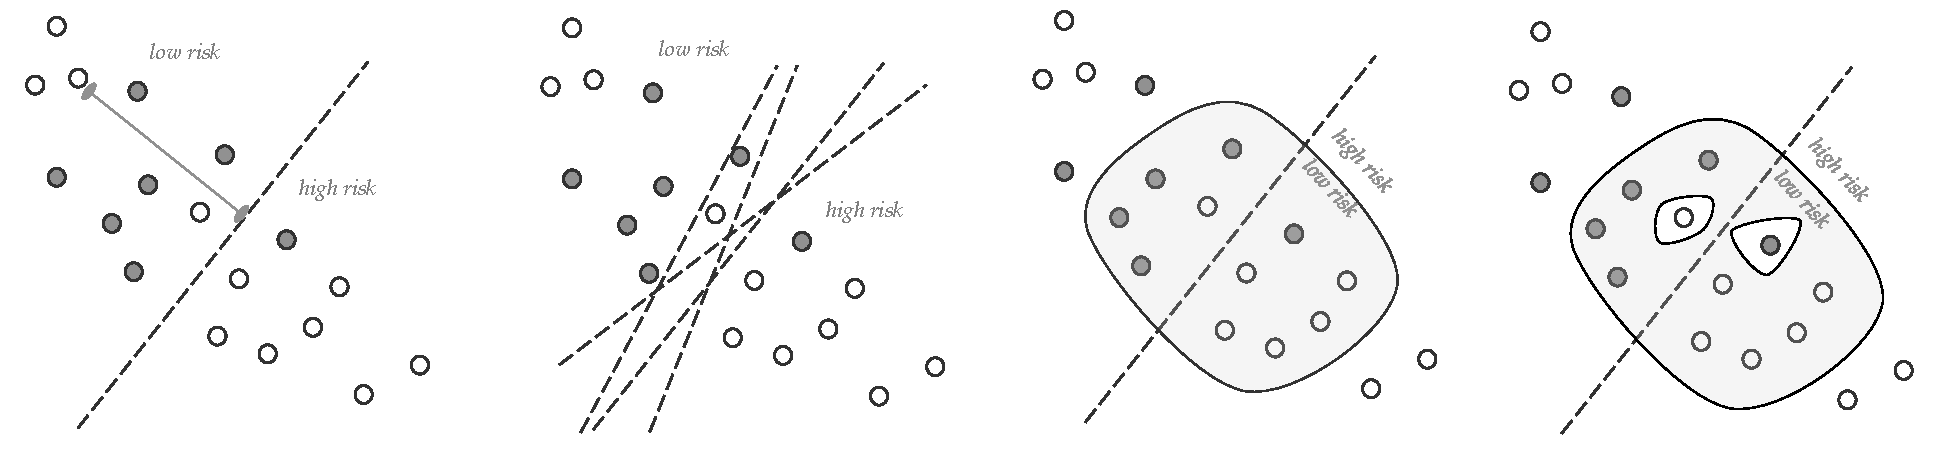
\includegraphics[width=\textwidth]{figures/active_learning.pdf}

\caption{Data is sampled from a Gaussian Mixture Model and in Fig. \ref{fig:subfigure1}, the red points are those that the trained policy, $\pi_{theta}$ will mis-predict. In Fig. \ref{fig:subfigure2} the One Class SVM is fit to the data and tries to estimate the areas of low risk (the light green region), while it is able to estimates the area where the majority of the data lies it also encloses the points the trained policy is mis-predicting. In Fig. \ref{fig:subfigure3}, the Risk Sensitive One Class SVM is able to effectively remove the red points from the region of low risk.}
\label{fig:support_example}
\end{figure*}


Let $\Phi$ be a feature map $\mathcal{X} \rightarrow \mathcal{F}$, i.e. a map into an inner product space $\mathcal{F}$ such that the inner product in the image of $\Phi$ can be computed by evaluating some  kernel

\vspace{-2ex}
\begin{align}
k(\bx_0,\bx_1) = \langle\Phi(\bx_0),\Phi(\bx_1)\rangle
\end{align}

such as the Gaussian kernel 

\vspace{-2ex}
\begin{align}
k(\bx_0,\bx_1) = e^{-||\bx_0 - \bx_1||^2/c}
\end{align}

The main idea is to solve an optimization problem that separates the origin, we solve the following quadratic problem:

\vspace{-2ex}
\begin{align}\label{eq:primal_sup}
\underset{w\in F, \mathbf{\xi} \in \mR, \rho \in \mR}{\mbox{min}}\: \frac{1}{2}||w||^2+\frac{1}{vn} \sum^n_i \xi_i - \rho\\
\mbox{s.t} \: \langle w,\Phi(x_i) \rangle \geq \rho - \xi_i, \: \xi_i \geq 0 \notag
\end{align}

The parameter $\nu$ controls the penalty on slack terms and asymptotically approaches is equivalent to $\gamma$ \cite{vert2006consistency}.  The decision function then becomes 

\vspace{-2ex}
\begin{align}\label{eq:decision_func}
g(x) = \mbox{sgn}(\langle w,\Phi(x) \rangle-\rho)
\end{align}

Where $g(x) = 1$ indicates in the support region and $(g) = -1$ denotes being outside the support region. The dual form of the optimization takes the form of a Quadratic Program with respect to the Gram Matrix \cite{scholkopf2001estimating}. 

Estimating the level set of a distribution can be a measure of the generalization ability of $\pi_{\theta}$ to points not within $\mathcal{D}$. However, it does not account for the fact that for a given $\theta$ or  solution to Eq. \ref{eq:super_objj}. $\pi_\theta$ may not correctly match the supervisor's controls for all points train on. To account for this, we propose a modification to the One Class SVM denote: 

\begin{align}
y_i = \left\{
     \begin{array}{lr}
       1 & : \pi_{\theta}(\bx_i) =\bu_i\\
       -1 & : \pi_{\theta}(\bx_i) \neq \bu_i
     \end{array}
   \right.
\end{align}

or $y_i$ is $1$ if the control applied matches the supervisor and $-1$ if it differs. In the regression case the decision between $1$ and $-1$ can be set by a some threshold on a L2-norm or $||\pi_{\theta}(\bx_i)-\bu_i||$. We use $y_i$ to modify the optimization as follows: 

\vspace{-2ex}
\begin{align}\label{eq:primal_sup}
\underset{w\in F, \mathbf{\xi} \in \mR^l, \rho \in \mR}{\mbox{min}}\: \frac{1}{2}||w||^2+\frac{1}{vn} \sum^n_i \xi_i - \rho\\
\mbox{s.t} \: y_i \langle w,\Phi(x_i)\rangle \geq \rho - \xi_i, \: \xi_i \geq 0 \label{eq:ineq}
\end{align}

Points that are mis-predicted are then enforced to lie on the opposite of the hyper-plane in the feature space $\phi(\bx)$, which carves out holes in the support region around them. The dual formulation, which is what is solved in practice, can be derived as 

\vspace{-2ex}
\begin{align}\label{eq:dual_sup}
\underset{\alpha\in \mathcal{R}}{\mbox{min}} \sum_i^n \sum_j^n \alpha_i\alpha_j y_i y_jk(\bx_i,\bx_j)\\
\mbox{s.t} \: 0 \leq \alpha \leq \frac{1}{\nu n} \:, \sum_i^n \alpha_i = 1 
\end{align}

Our decision boundary function $g(\bx)$ is then derived in terms of the support vectors as $g(\bx) = \sum_i^n \alpha_i y_i k(\bx_i,\bx) - \rho$. To compute the $\rho$ term,we leverage the fact that for an optimal solution the inequalities in Eq. \ref{eq:ineq} are equal for any $\alpha_j$ such that $0 < \alpha_j < \frac{1}{\nu n}$. Therefore we can compute $\rho$ as  $\rho = \sum_i^n y_i \alpha_i k(\bx_i,\bx_j)$ \cite{scholkopf2001estimating}. 




\subsection{SHIV: SVM-Based Reduction in Human Intervention}

Our proposed method trains a policy, $\pi_{\theta_k}$, but also estimates where the policy is likely to accurately predict the supervisor's control,which we define as the region of low risk.  In the statistics community, a known property is that estimators are function will likely mis-classify if they are evaluated at points not in the distribution sampled from.Techniques such as importance sampling use this results to train estimators on data drawn from a different distribution \cite{tokdar2010importance}.  Thus, we try to estimate the level set of the training distribution, which is explained in \ref{sec:level} and only have the supervisor provide labels when the robot leaves this boundary. Furthermore to avoid entering pathological states that are far from the supervisor's demonstrations, we terminate the roll-out when it is a certain distance or risk factor from the decision boundary, which is given by $r(\bx) = \sum_i^n \alpha_i \bx_i k(\bx_i,\bx)-\rho$. The risk threshold, $r_0$, is user defined based on the task. 

\subsubsection{Step 1}
Similar to DAgger at iteration $k$ the algorithm estimates a policy, $\pi_{\theta_k}$ on the dataset $\mathcal{D}_k$ by solving Eq. \ref{eq:super_objj}. We then estimate the level set of the distribution being trained on by solving the optimization for the One Class SVM or $\ref{eq:primal_sup}$ on the dataset $\mathcal{D}_k$. We now have a decision boundary $g_k(\bx)$, which is $1$ if the region is in the low risk area and $-1$ otherwise . The parameter $\nu$ is an estimate of how much probability mass is contained in the level set and can be use to control the size of the low risk region. 
 
 
 \subsubsection{Step 2}
 In DAgger the policy that was rolled out is $\pi_{\theta_k}$, however this could potential encounter pathological states that are far from the initial set of demonstrations $\mathcal{D}_0$. To prevent this we terminate the rolled out policy if the risk, or distance from the support, is above some threshold $r(\bx_t) > r_0$.  Furthermore, instead of labeling every state now the supervisor is only require to label states outside of the level set or $\bx$, where $g(\bx) = -1$.  These states are then added to the dataset $\mathcal{D}_{k}$


\section{Experiments}
\subsection{Driving Example}
A common benchmark in Reinforcement Learning  is a car driving around a track avoiding other cars \cite{argall2009survey}. To illustrate our methods ability in high dimensions, the car must follow a polygonal track using only HOG features extracted from images. If the car falls off the track, it is placed back on the center facing the angle of the polygonal track piece. We sample the polygonal track by drawing points from a Gaussian with a mean that is the centered of the video game work space. The convex hull of the sampled points is then computed. The car's control space $u = \lbrace -15^\circ, 0, 15^\circ \rbrace$ or 3 discrete commands that change the angle of the car. The internal state space of the car is xy-coordinates and the angle it is facing. Our supervisor is a solver that uses state space search through the driving simulator to plan the next control.

We have the supervisor drive around the track 2 times and then collect the raw images observed. We use a Gaussian Pyramids to down sample the images to $125 \times 125$ RGB pixels and then extract Histogram of Oriented Gradients (HOG) features using OpenCV,  where the size of $\bx$ is $27926$. For both DAgger and SHIV, we use a Linear Support Vector Machine (SVM) as the policy representation, with the regularization term on the slack variable $\gamma=0.01$, which was set via cross validation on the initial training examples from our expert. For the optimization of Eq. \ref{eq:dual_sup} in SHIV we used a radial basis function as well for the kernel with a bandwidth of $\lambda=0.01$ and $\nu = 0.95$ to account for $95\%$ of the training distribution. 

To compare our method against a traditional confidence based active learning approach, we use a confidence measure  of distance from the hyperplane. The threshold was set to the average distance from the hyperplane for the mis-classified points in $\mathcal{D}_0$, which consisted of two demonstrations from our solver. We measured the performance of our modified One Class SVM to the confidence measure, in terms of how many states are estimated to be of low risk (i.e. correctly classified) and are of actually high risk on the first policy roll out. Results  are averaged over 50 tracks and shown in Table \ref{table:active_comp}. 


We compare performance in terms of minimization of the underlying cost function $c(\bx,\bu)$, which is the  number of times the car left the track versus the number of queries made to the supervisor. In Fig. \ref{fig:car_cost}, we plot the performance of DAgger, SHIV and SHIV using only the traditional One-Class SVM without the modification.  Initial results, which are run for 6 iterations each and are averaged over 40 levels, shown in Fig. \ref{fig:car_cost} suggest a $70\%$ reduction in the number of queries needed for SHIV compared to DAgger. 
 

\begin{figure}[t]
\centering
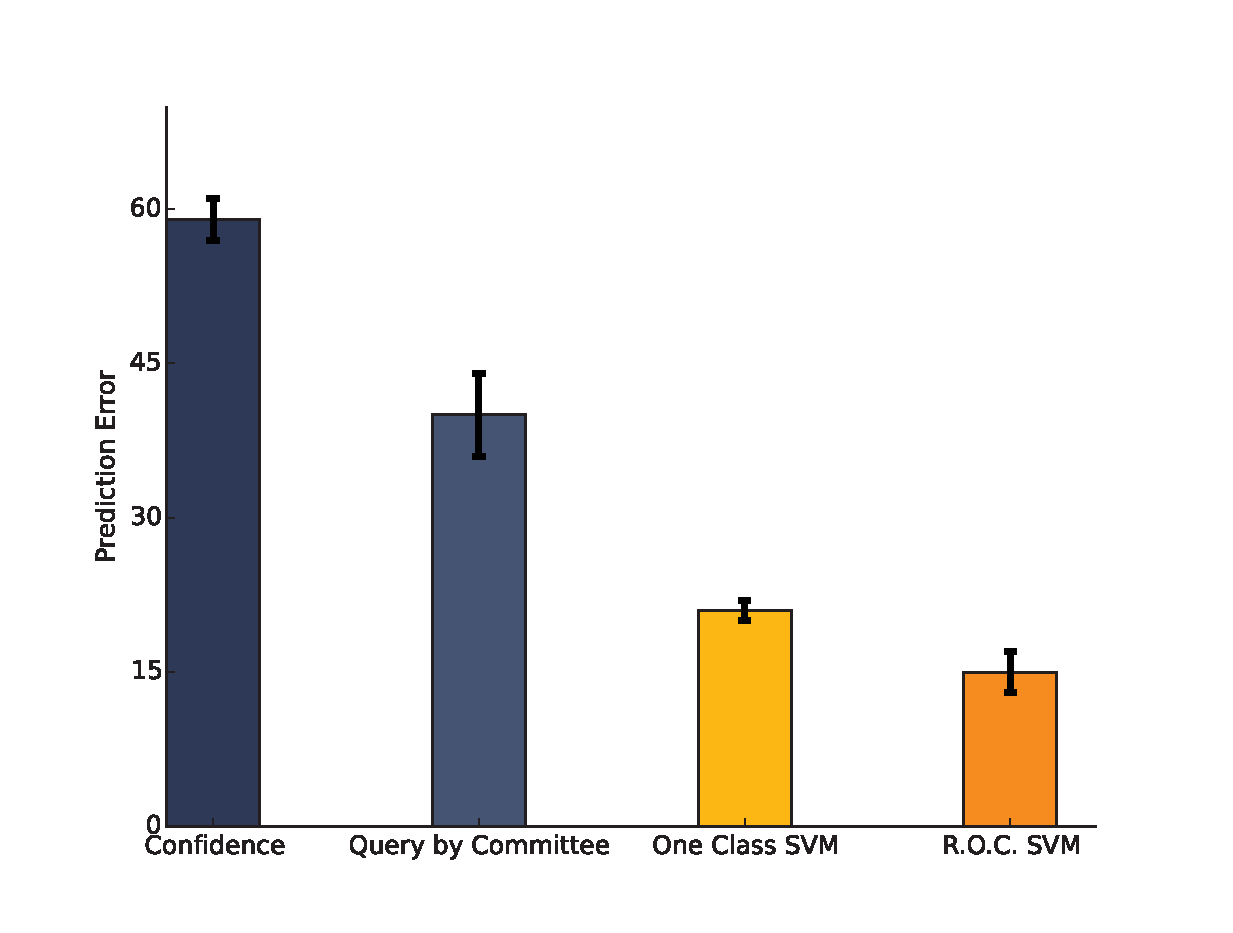
\includegraphics[width=9cm, height=8cm]{figures/risk_bar.eps}
   \caption { \footnotesize  To compare our method against a traditional confidence based active learning approach, we use a confidence measure  of distance from the hyperplane. The threshold was set to the average distance from the hyperplane for the mis-classified points in $\mathcal{D}_0$, which consisted of two demonstrations from our solver. We measured the performance of our modified One Class SVM to the confidence measure, in terms of how many states are estimated to be of low risk (i.e. correctly classified) and are of actually high risk on the first policy roll out. Results  are averaged over 50 randomly generated tracks. 
   }

\label{fig:active_comp}
\end{figure}



\begin{figure}[t!]
\centering
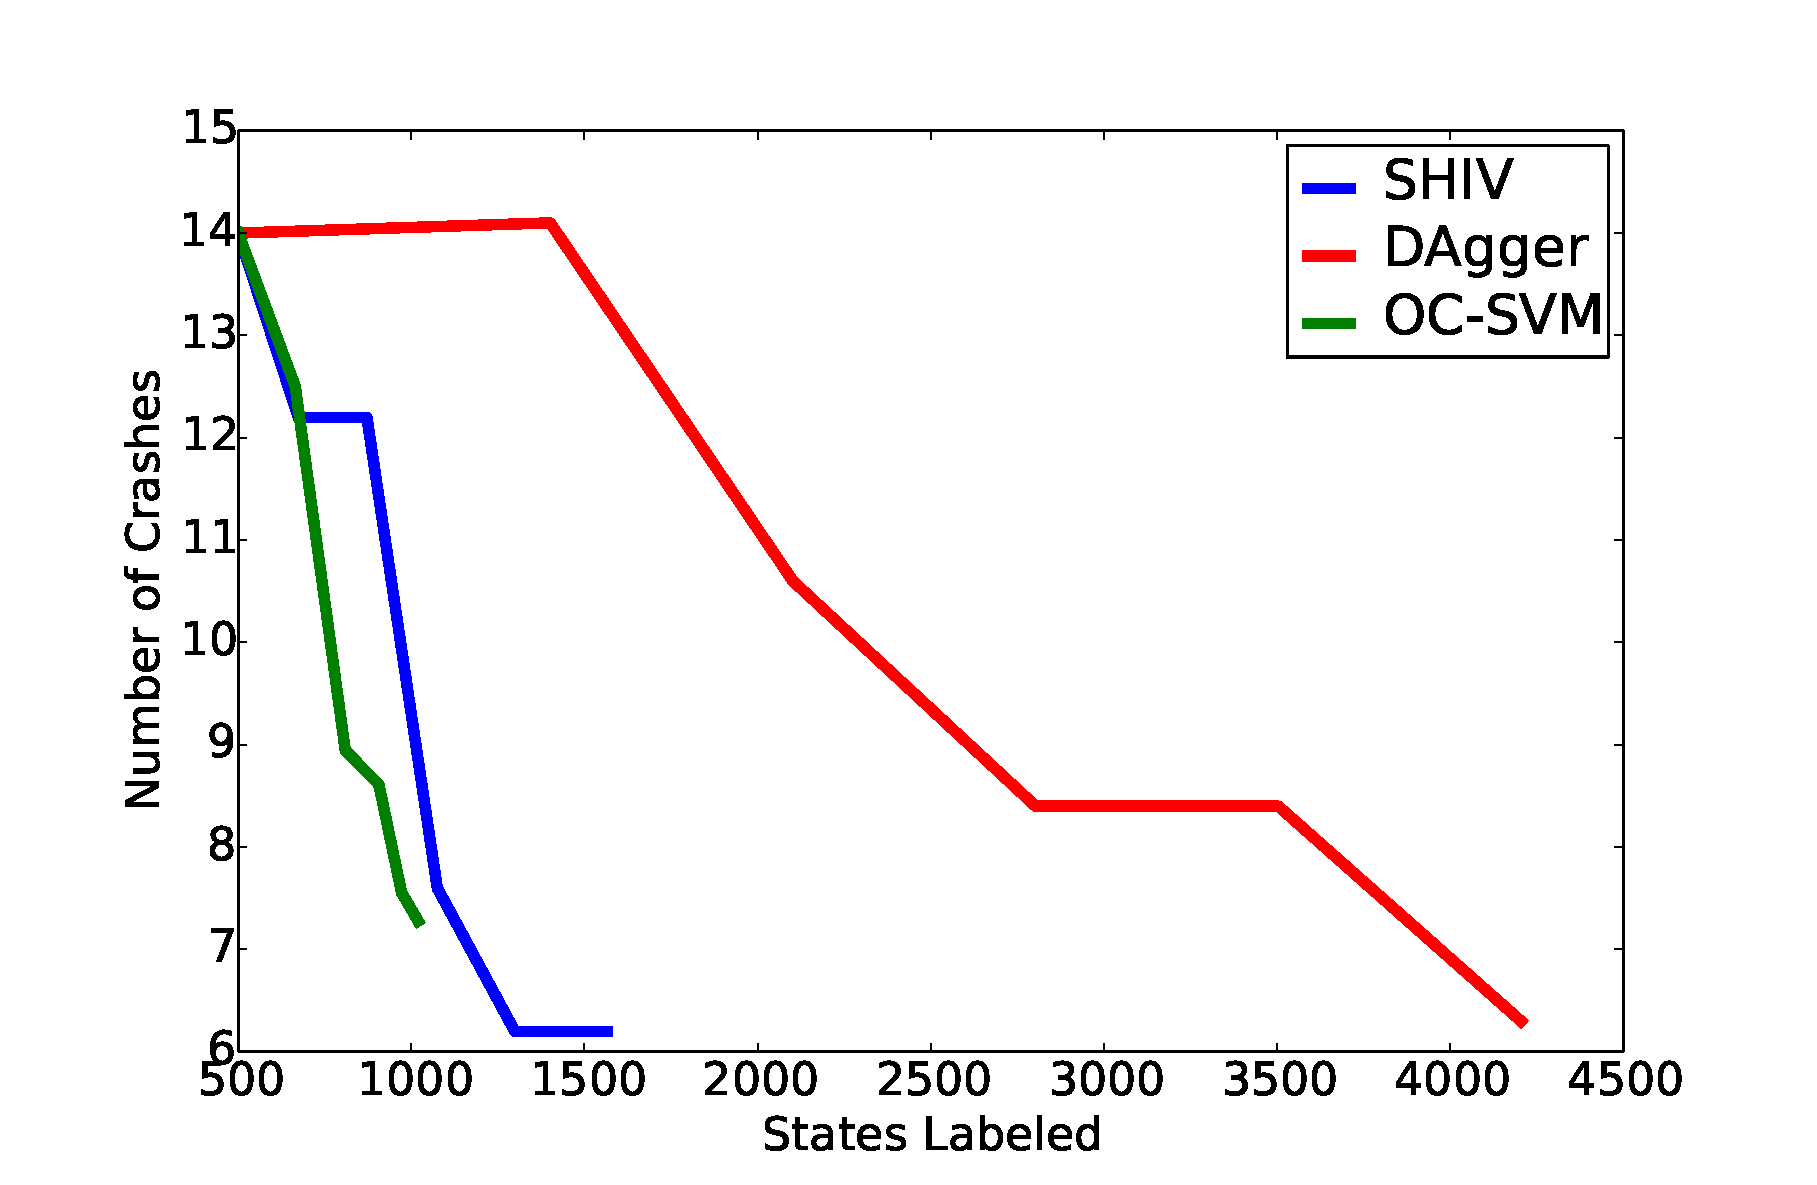
\includegraphics[width=8cm, height=6cm]{figures/dagger_shiv_one_class.eps}
\caption{We compare performance in terms of minimization of the underlying cost function $c(\bx,\bu)$, which is the  number of times the car left the track versus the number of queries made to the supervisor. In Fig. \ref{fig:car_cost}, we plot the performance of DAgger and SHIV.  Initial results, which are run for 6 iterations each and are averaged over 40 levels, shown in Fig. \ref{fig:car_cost} suggest an $70\%$ reduction in the number of queries needed for SHIV compared to DAgger,}
\vspace*{-10pt}
\label{fig:car_cost}
\end{figure}


\subsection{Grasping In Clutter}
To illustrate how our technique can be used in the continuous case and with a human demonstrator. 
We look at having a human demonstrator control a robot arm in 2D to reach a target object with out knocking other objects off a table. We used Box2D a physics simulator to model the virtual world. The arm, shown in Fig. \ref{fig:box2d_arm}, consists of 3 degrees of freedom and has a parallel jaw gripper. For input the human demonstrator provides controls through an XBox controller. The left and right joystick determined the x and y velocity of the center of the end effector. The left bumper of the controller provided a binary input for opening and closing the gripper. 

\todo{double check this section with Sammy}
Our state $\bx$ consisted of the 3 dimensional pose of the six objects on the table (translation and rotation), the 3 joint angles of the arm and a scalar value in the range $[0,1]$ that measured the position of the gripper, 1 being opened and zero being closed. For our representation of $\pi_{\theta}$, we used linear ridge regression. We defined two cost functions, $C(\bx,\bu)$, as the sum of the number of objects knocked off the table and 1 for not successfully grasping the target object. 

In experiment, we had our human demonstrator provide one demonstration and then iterated both  DAgger and SHIV until the cost function was zero during the policy roll out. At each iteration, we sampled the pose of the target object from an isotropic Gaussian with a standard deviation that is equal to $3\%$ of the width of the table. 

In Figure , we show both the cost function associated with knocking an object off the table and the one associated with being able to successfully grasp an object or not. \todo{Finalize results then discuss them}




\subsection{Surgical Experiment}
\todo{Need help discussing this better}
In this experiment, we look at the task of inserting a needle into tissue in preparation for suturing. Needle insertion can be a challenging task for surgeons and learning a controller to do so could alleviate some of the burden placed on surgeons. We collected data from a surgeon, Dr. Douglas Boyd, on the Da Vince Research Kit. 

Dr. Boyd demonstrated a series of trajectories that started at an initial attempted needle insertion pose and applied the neccesary corrections to achieve a correct pose. We used three of these demonstrations as our initial dataset $\mathcal{D}_0$. Dr. Boyd couldn't be around for the interactive labeling of both SHIV and DAgger, so we had to hardcore and expert controller that computed the transformation between the desired insertion pose and the current pose. We did this by calculating the inverse of a transformation matrix. 

\begin{figure}[t!]
\centering
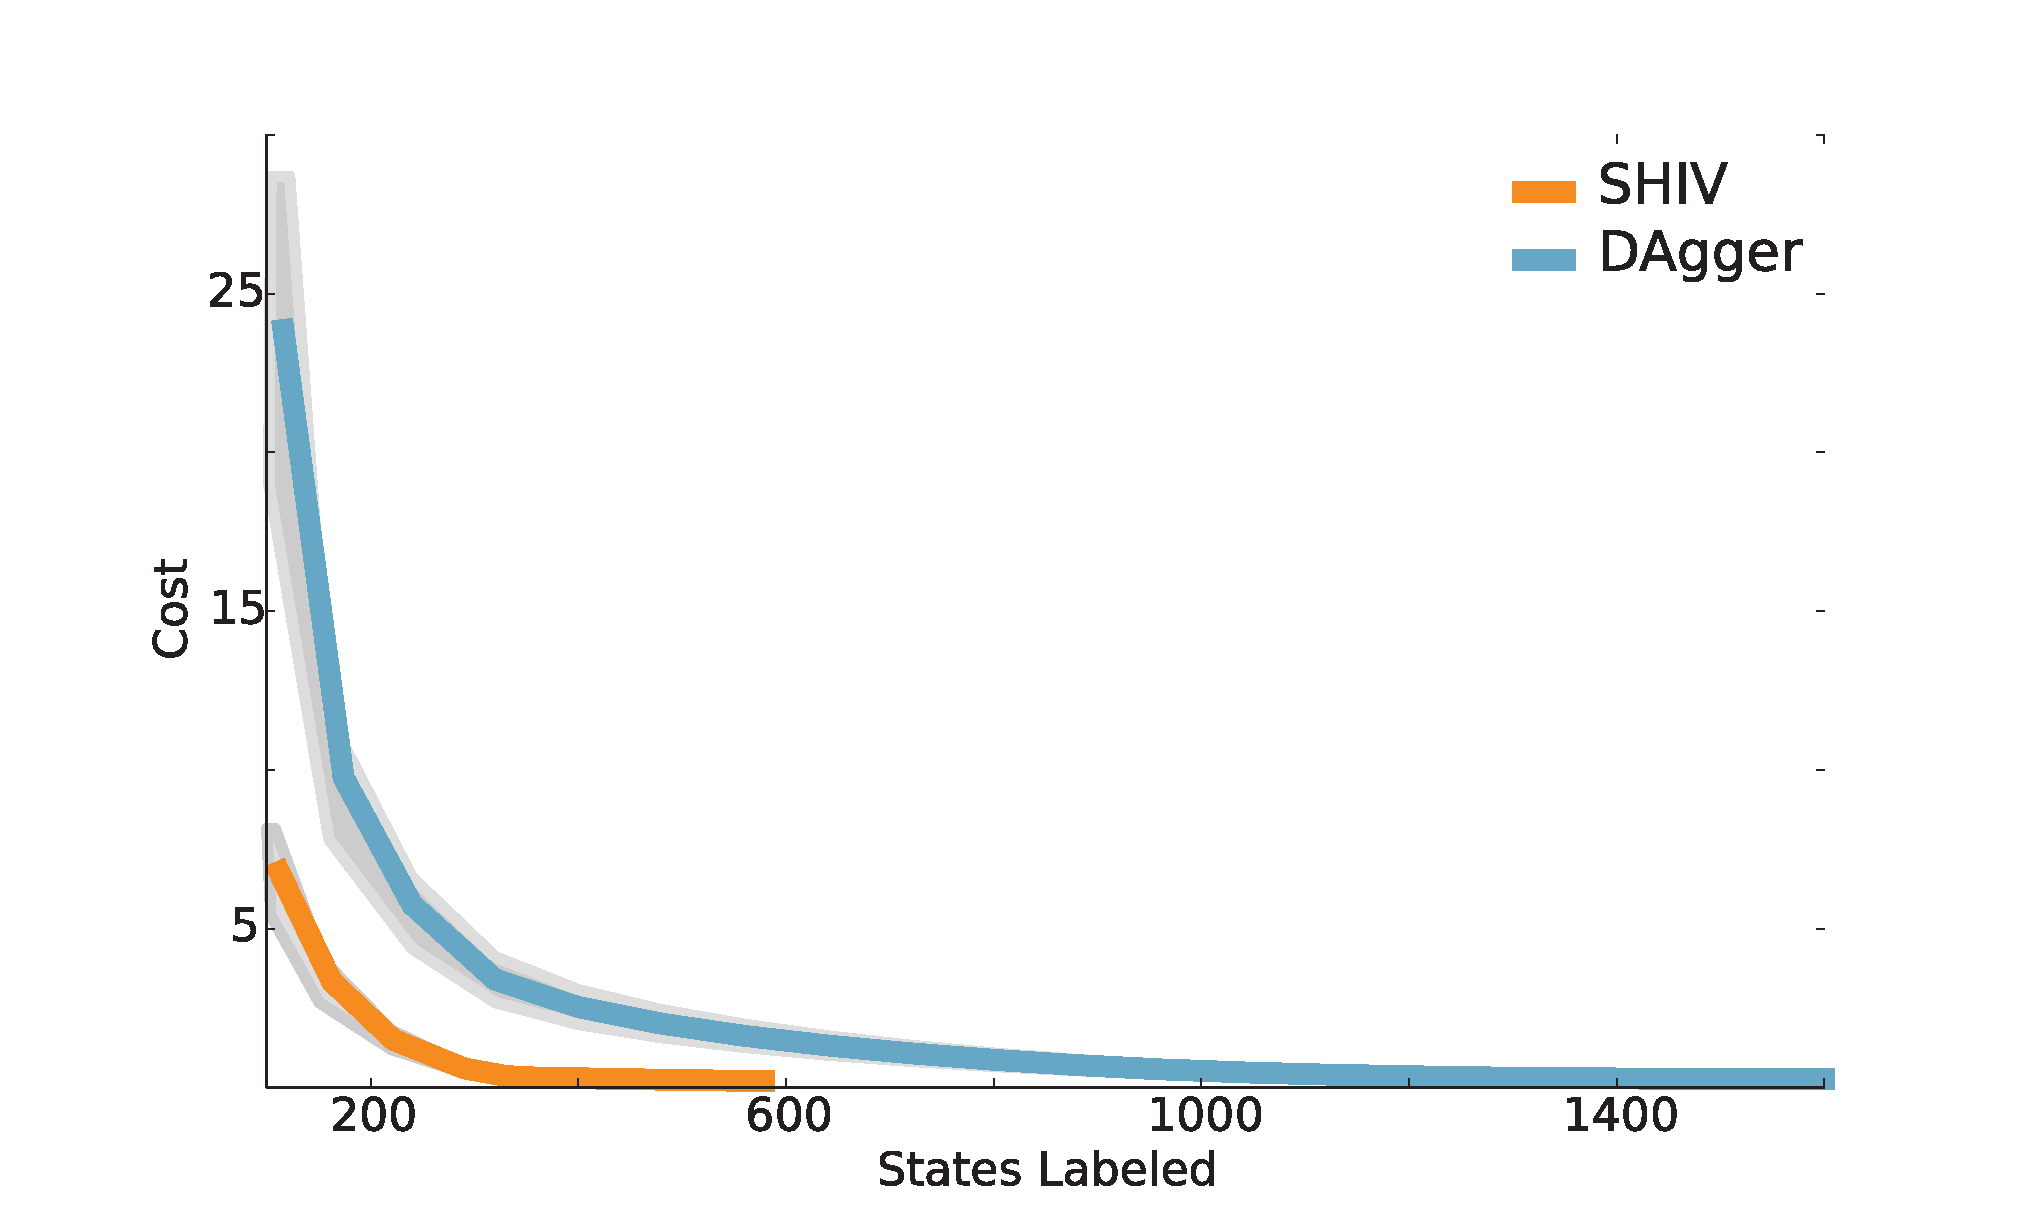
\includegraphics[width=\columnwidth, height=6cm]{figures/needle_insertion_results.eps}
\caption{We compare performance in terms of minimization of the underlying cost function $c(\bx,\bu)$, which is euclidean distance between translation in centimeters. In Fig. \ref{fig:car_cost}, we plot the performance of DAgger, SHIV and SHIV using only the traditional One-Class SVM without the modification.  Initial results, which are run for 20 iterations each and are averaged over 40 different initial starting positions, shown in Fig. \ref{fig:car_cost} suggest an $67\%$ reduction in the number of queries needed for SHIV compared to DAgger,}
\vspace*{-10pt}
\label{fig:car_cost}
\end{figure}



\section{Discussions and Future Work}
SHIV currently provides a way to apply active learning to online imitation learning, however its use of level set estimation of the underlying distribution introduces several hyper parameters. As Fig. shown these can significantly effect performance if not tuned correctly. Future work will look at using cross validation on a hold out set of data to more effectively tune parameters. 

Another potential issue is that each iteration of SHIV requires solving a quadratic program with the Gram matrix. As we scale to harder tasks that require significantly more data, this can become problematic. Future work will look at using techniques like PCA and random feature projections to scale efficiently \todo{cite something}. 

Lastly, our approach is promising in simulation. However we need to evaluate how our active learning method will work on a real robot with noisy sensor observations. Future work will be doing the grasping in clutter experiments on an actual robot. 

\section{Acknowledgments} 
This work is supported in part by the U.S. National Science Foundation under Award IIS-1227536 and NSF-Graduate Research Fellowship.. 
We thank UC Berkeley and our colleagues who gave feedback and suggestions, in particular Sanjay Krishnan, Siddarth Sen, Steve McKinley and Sergey Levine.




\bibliographystyle{IEEEtranS}
\bibliography{references}



\end{document}
